
\section{Durchführung}
Zuerst werden die zwei runden und zwei eckigen Stäbe unterschiedlichen Materials vermessen und gewogen.

\noindent
Der Versuchsaufbau ist in Abbildung (\ref{fig:aufbau}) dargestellt.

\begin{figure}
    \centering
       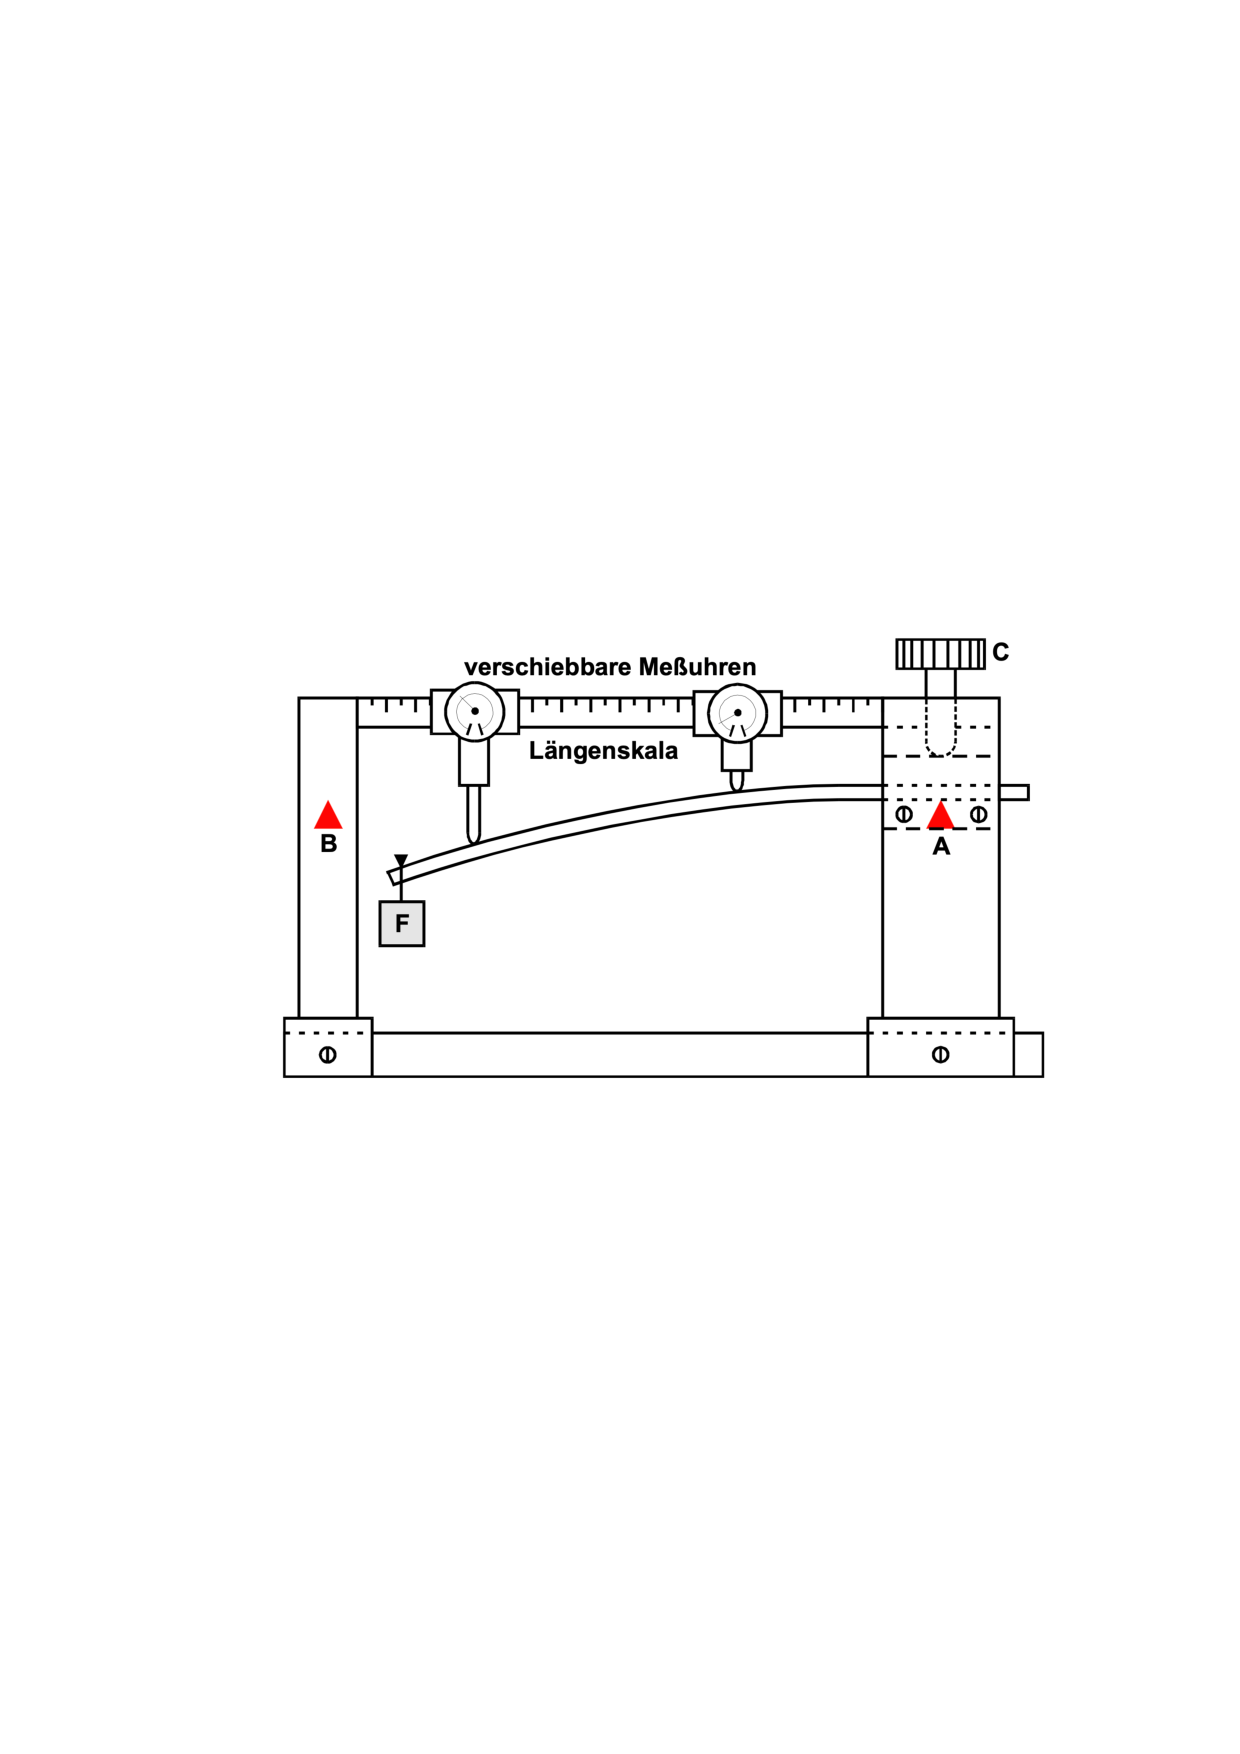
\includegraphics[height=5cm]{aufbau.pdf}
       \caption{Aufbau zur Bestimmung des Elastizitätsmoduls (Quelle: \cite{V103}).}
       \label{fig:aufbau}
\end{figure}

\noindent
Zur Untersuchung der einseitigen Einspannung wird der Stab im Punkt B befestigt.
Die beiden Messuhren werden tariert und die Masse wird an das nicht eingespannte Ende bei $x=52 \si{\centi\meter}$ eingehangen.
Nach kurzer Zeit kann die Durchbiegung an den beiden Messuhren sowie deren Position an der Skala abgelesen werden.
Die Masse wird abgehängt und die Positionen der Messuhren wird verändert.
Der Vorgang wird widerholt, bis zehn Wertepaare aufgenommen wurden.

\noindent
Für die beidseitige Einspannung wird der Stab zusätzlich auf Punkt B aufgelegt.
Die beiden Messuhren werden tariert und die Masse wird in die Mitte bei $x=27.5 \si{\centi\meter}$ eingehängt.
Analog zur einseitigen Einspannung wird die Durchbiegung und Position abgelesen, die Masse abgehängt, die Messuhren verschoben und der Vorgang viermal wiederholt.

\noindent
Beide Verfahren werden für alle vier Stäbe durchgeführt.
